\chapter{Conclusiones y trabajo futuro}
\label{chap:5}

\section*{Conclusiones}

En esta tesina se ha presentado una novedosa técnica de minería de procesos mediante un enfoque
supervisado basado en dominios numéricos abstractos y el uso de resolvedores de satisfacibilidad 
módulo teorías que permite, mediante el uso de información negativa, obtener, simplificar y
generalizar modelos de procesos a partir de un log de eventos. Esta información negativa puede provenir 
de un un log con trazas prohibidas (i.e. comportamientos que el sistema \emph{no} debe ejecutar),
derivada artificialmente o de conocimiento experto.

Este trabajo utiliza un concepto fundamental como es el de supervisar (ya sea manual o automáticamente)
las técnicas de minería de procesos de manera de mejorar la calidad de los modelos derivados de
su aplicación. Se presenta como extensión a las técnicas propuestas en~\cite{CarmonaC14}
y~\cite{LeonCB15}, las cuales presentan diferentes falencias que han sido resueltas mediante
este nuevo enfoque.

Además, como parte de esta tesina, se desarrolló íntegramente una herramienta de
minería de procesos llamada \pachtool.
Esta nueva herramienta%, ideada para estudiar el comportamiento del nuevo enfoque, 
permite obtener un modelo para un cierto proceso a partir de un log de eventos del mismo.
Como algoritmo de descubrimiento, la herramienta acepta diferentes formatos del log 
e implementa ciertas técnicas de alto nivel que permiten el manejo de logs de gran 
tamaño de manera rápida y efectiva.
Por otra parte, \pachtool permite generalizar y simplificar modelos de procesos presentados como
una red de Petri de manera supervisada mediante el uso de información negativa. Este 
post procesamiento no necesariamente debe ser aplicado sobre los modelos generados por \pachtool,
sino que también pueden aplicarse sobre modelos obtenidos por otras herramientas de descubrimiento.

En la \autoref{fig:allsimp} puede observarse un ejemplo donde visualmente se aprecian los beneficios del
uso de la metodología introducida.

\begin{figure}[H]
    \centering
    \subbottom[\label{sfig:allsimp.1}\tiny\pachtool y teoría de poliedros]{\scalebox{.04}{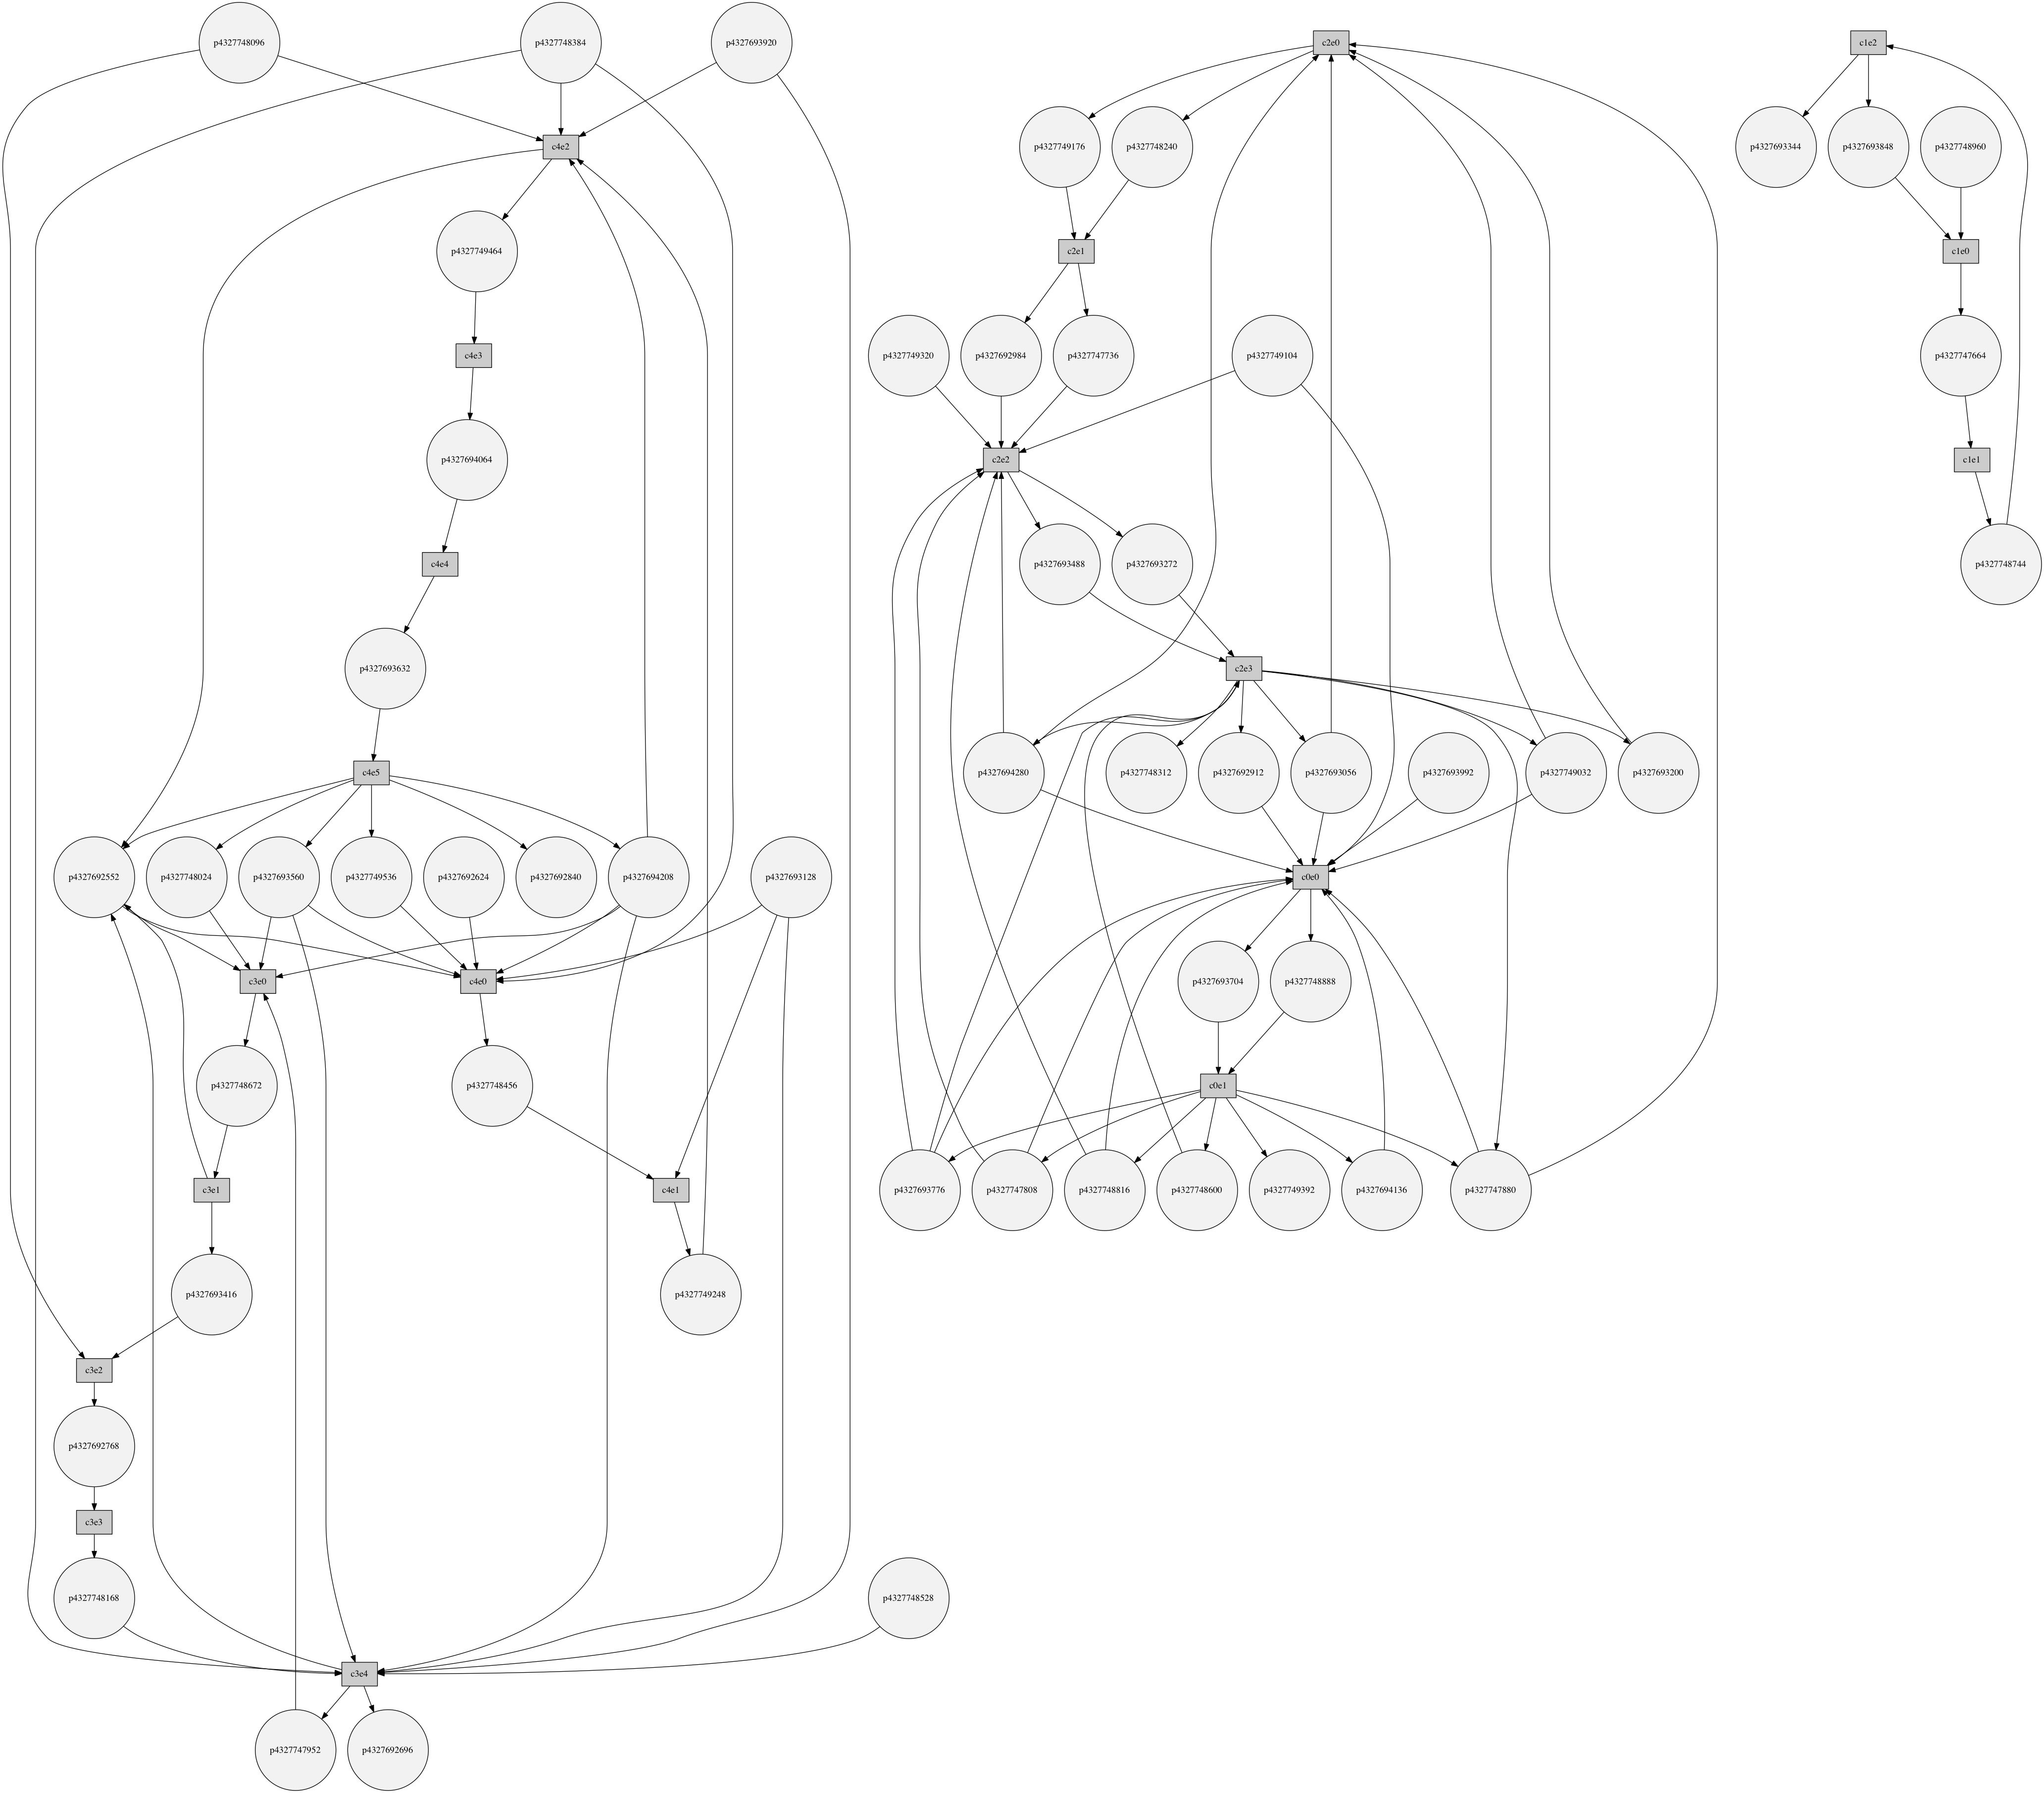
\includegraphics{img/cycles-pol}}}
    \hspace{1cm}
    \subbottom[\label{sfig:allsimp.2}\tiny\textsc{Removal} sobre~\autoref{sfig:allsimp.1}]{\scalebox{.05}{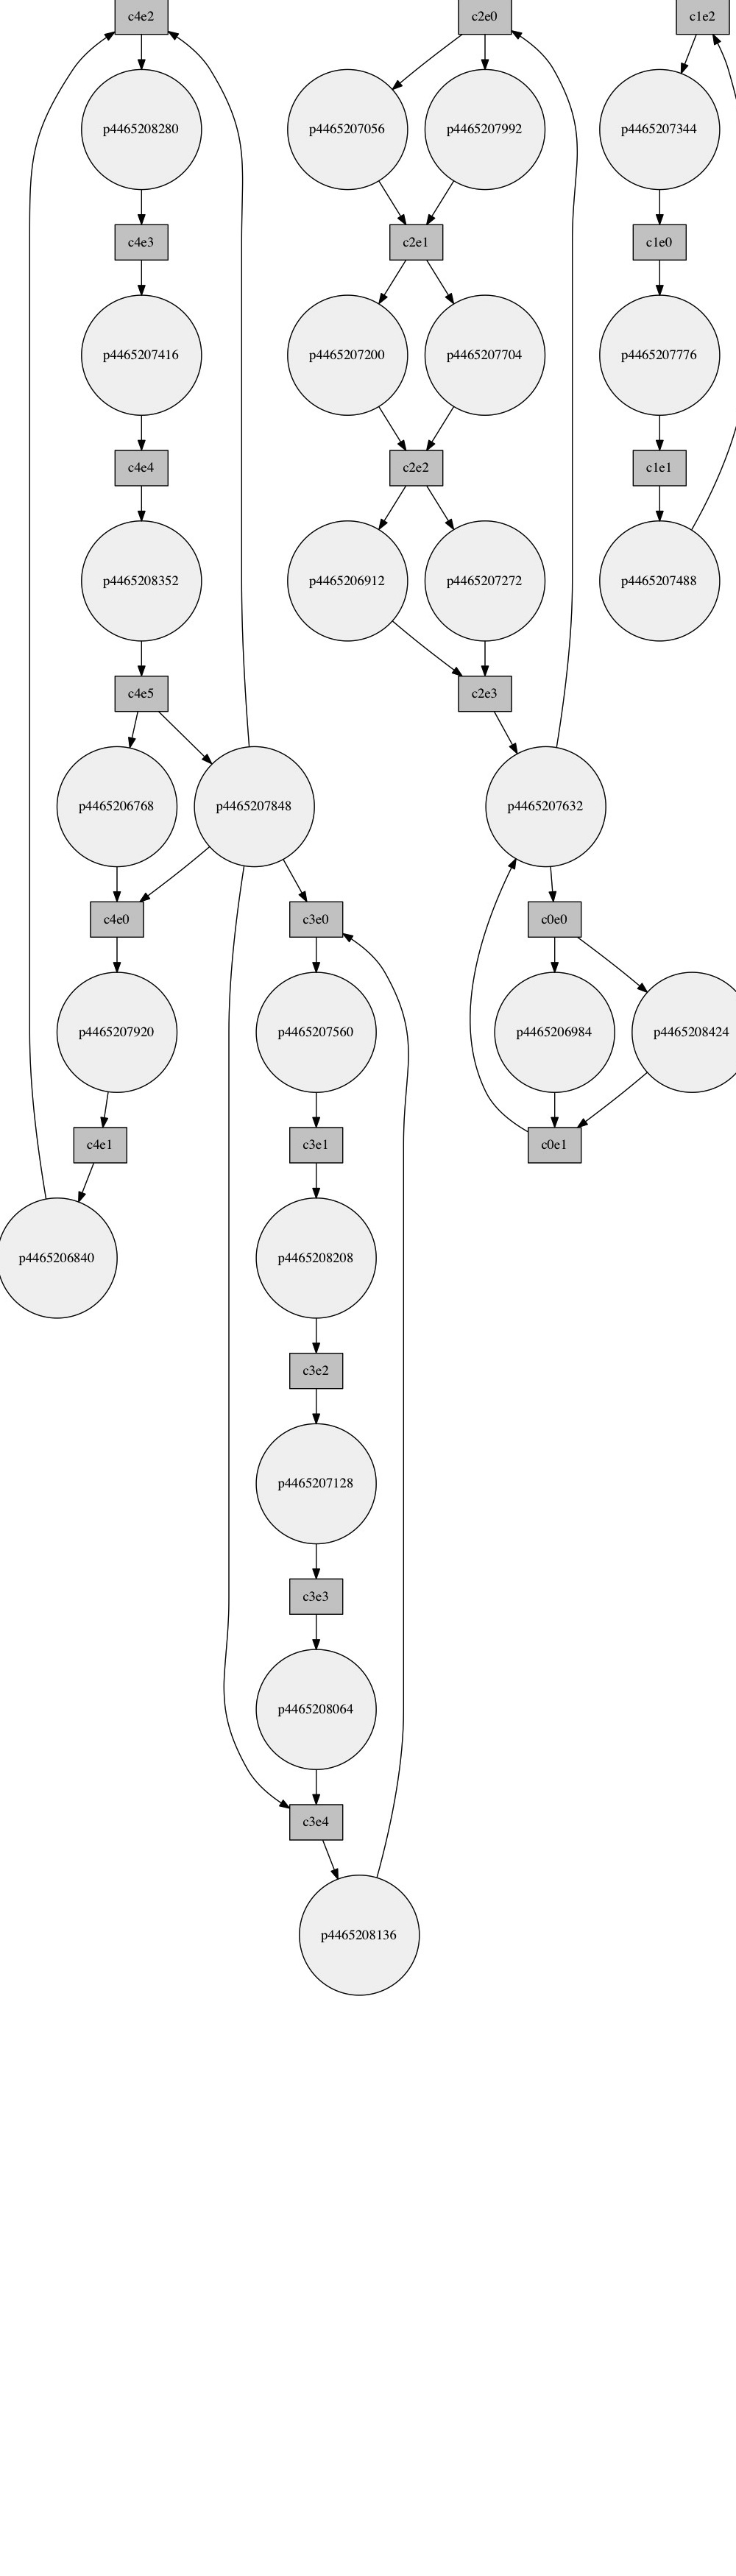
\includegraphics{img/cycles-pol-rem}}}
    \subbottom[\label{sfig:allsimp.3}\tiny Enfoque de~\cite{Murata89}]{\scalebox{.04}{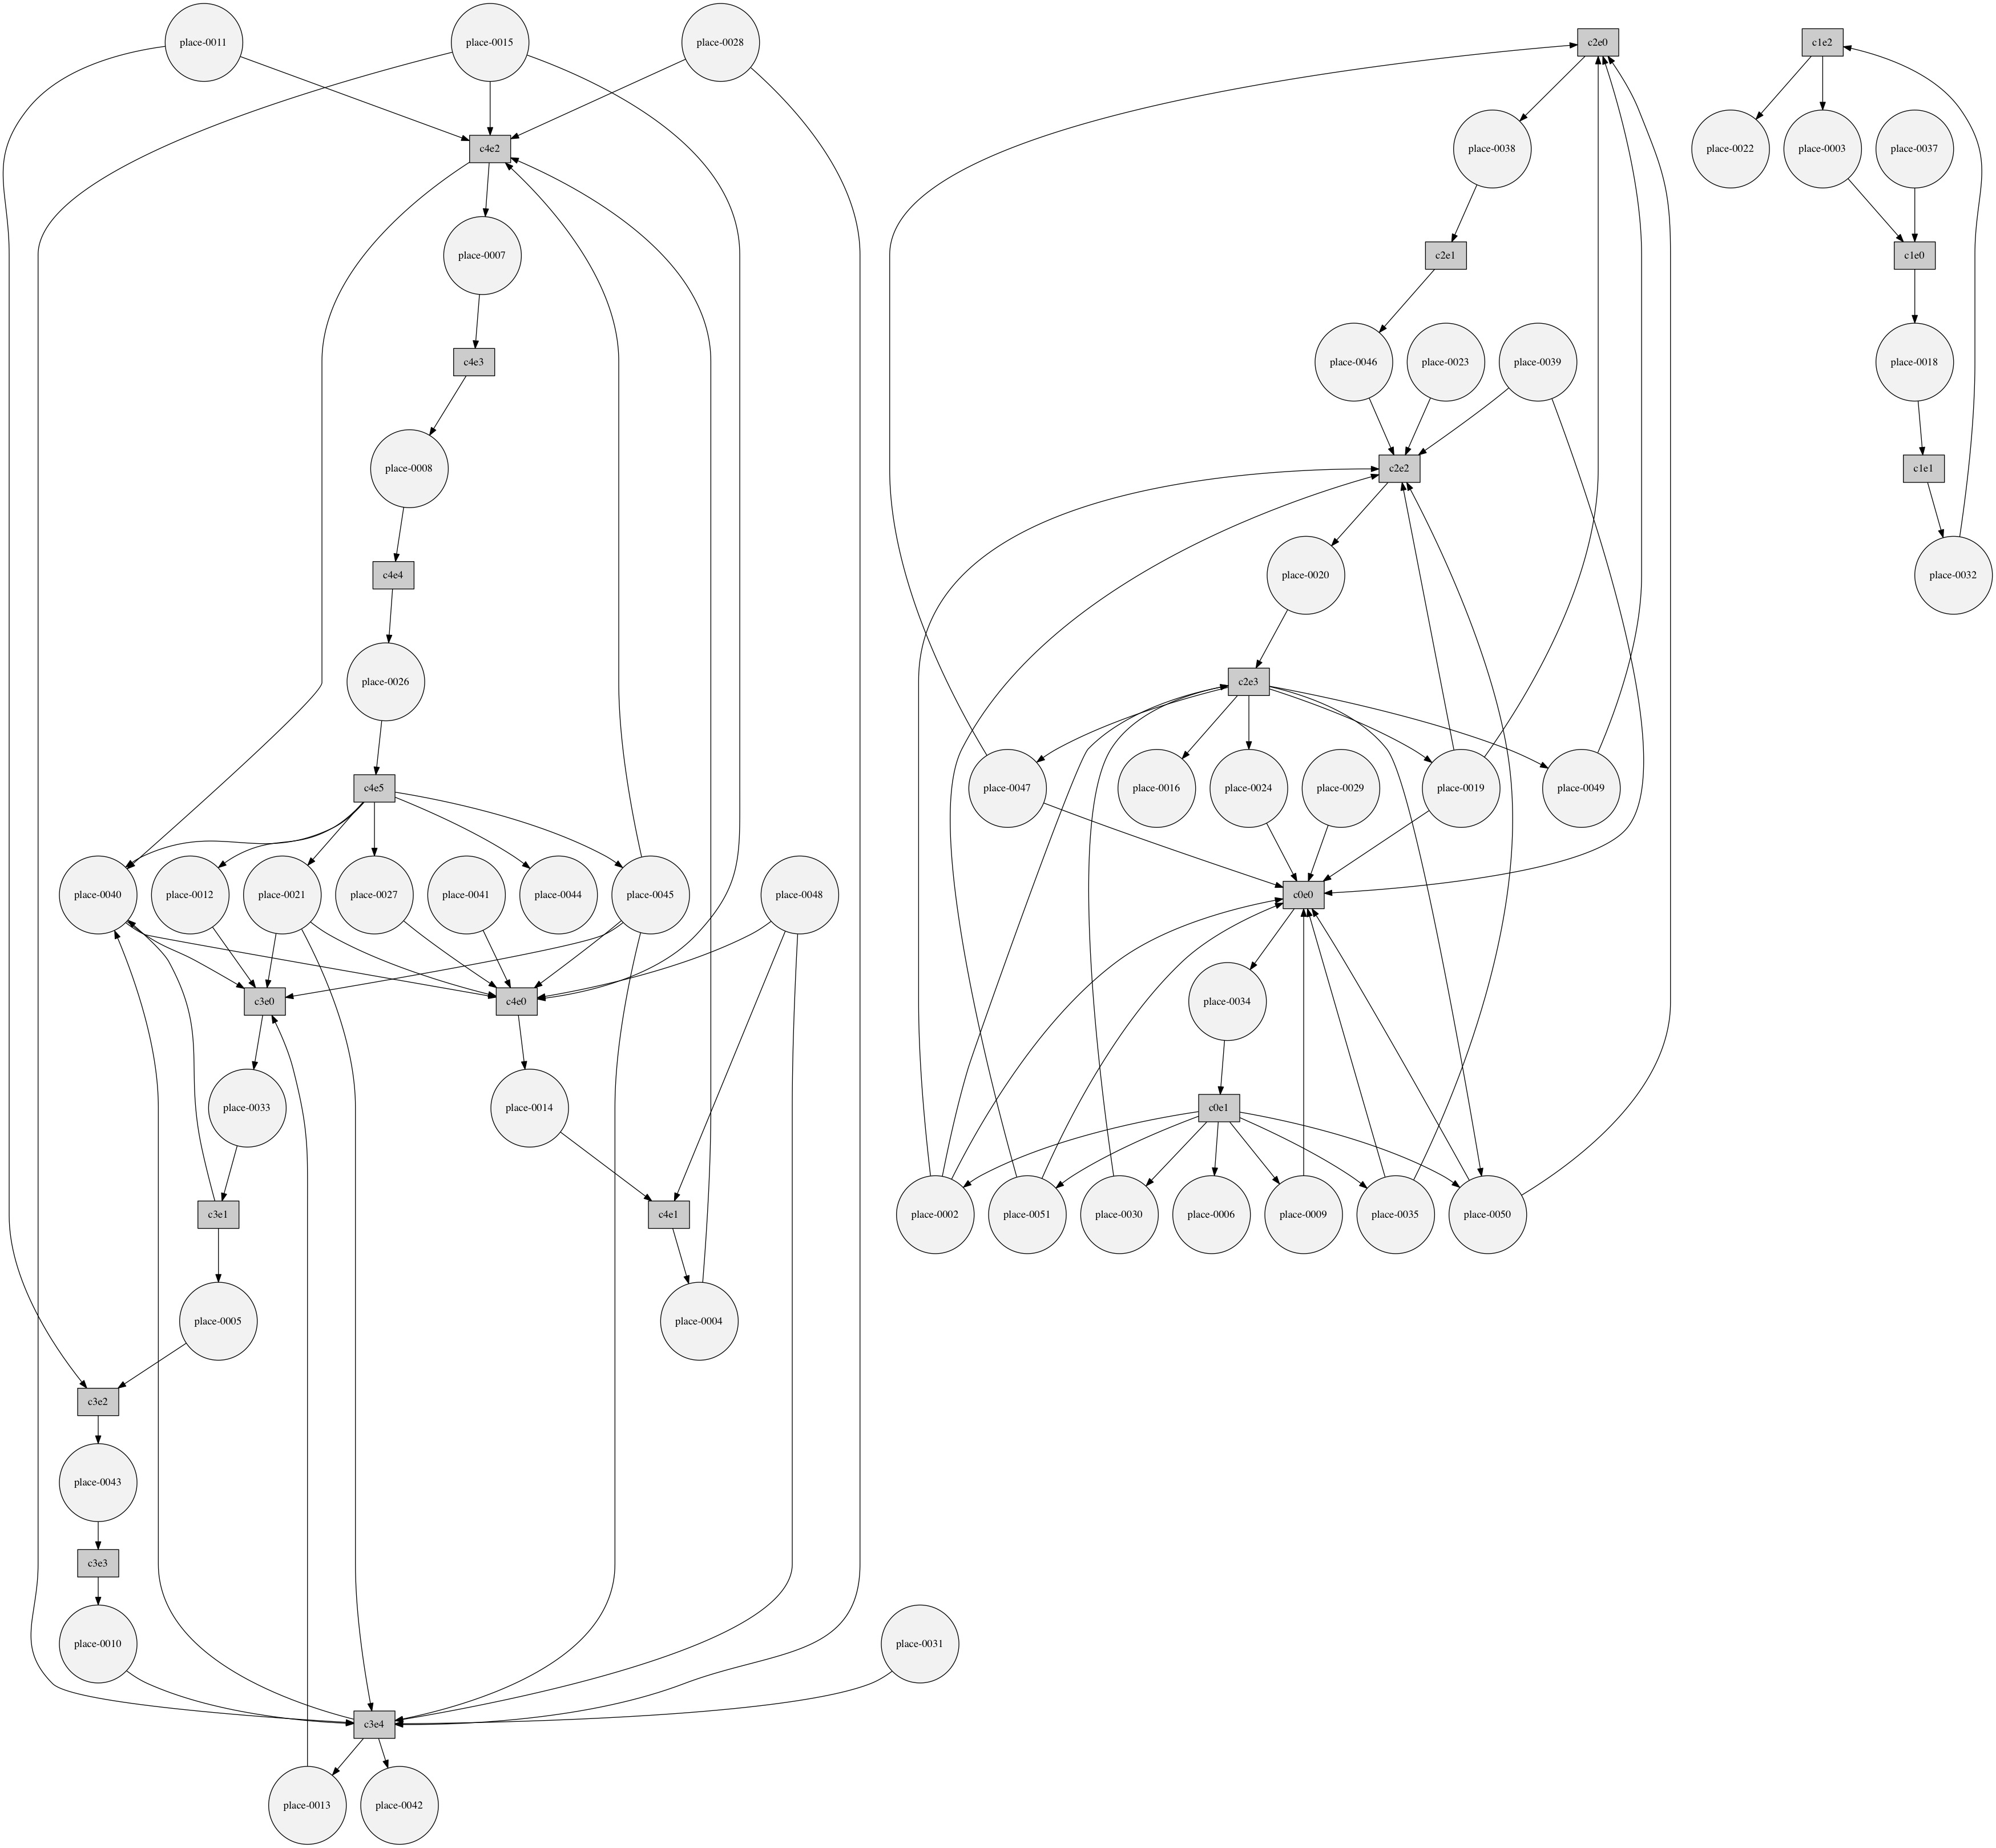
\includegraphics{img/cycles_murata}}}
    \hspace{7mm}
    \subbottom[\label{sfig:allsimp.4}\tiny Enfoque de~\cite{LeonCB15}]{\scalebox{.04}{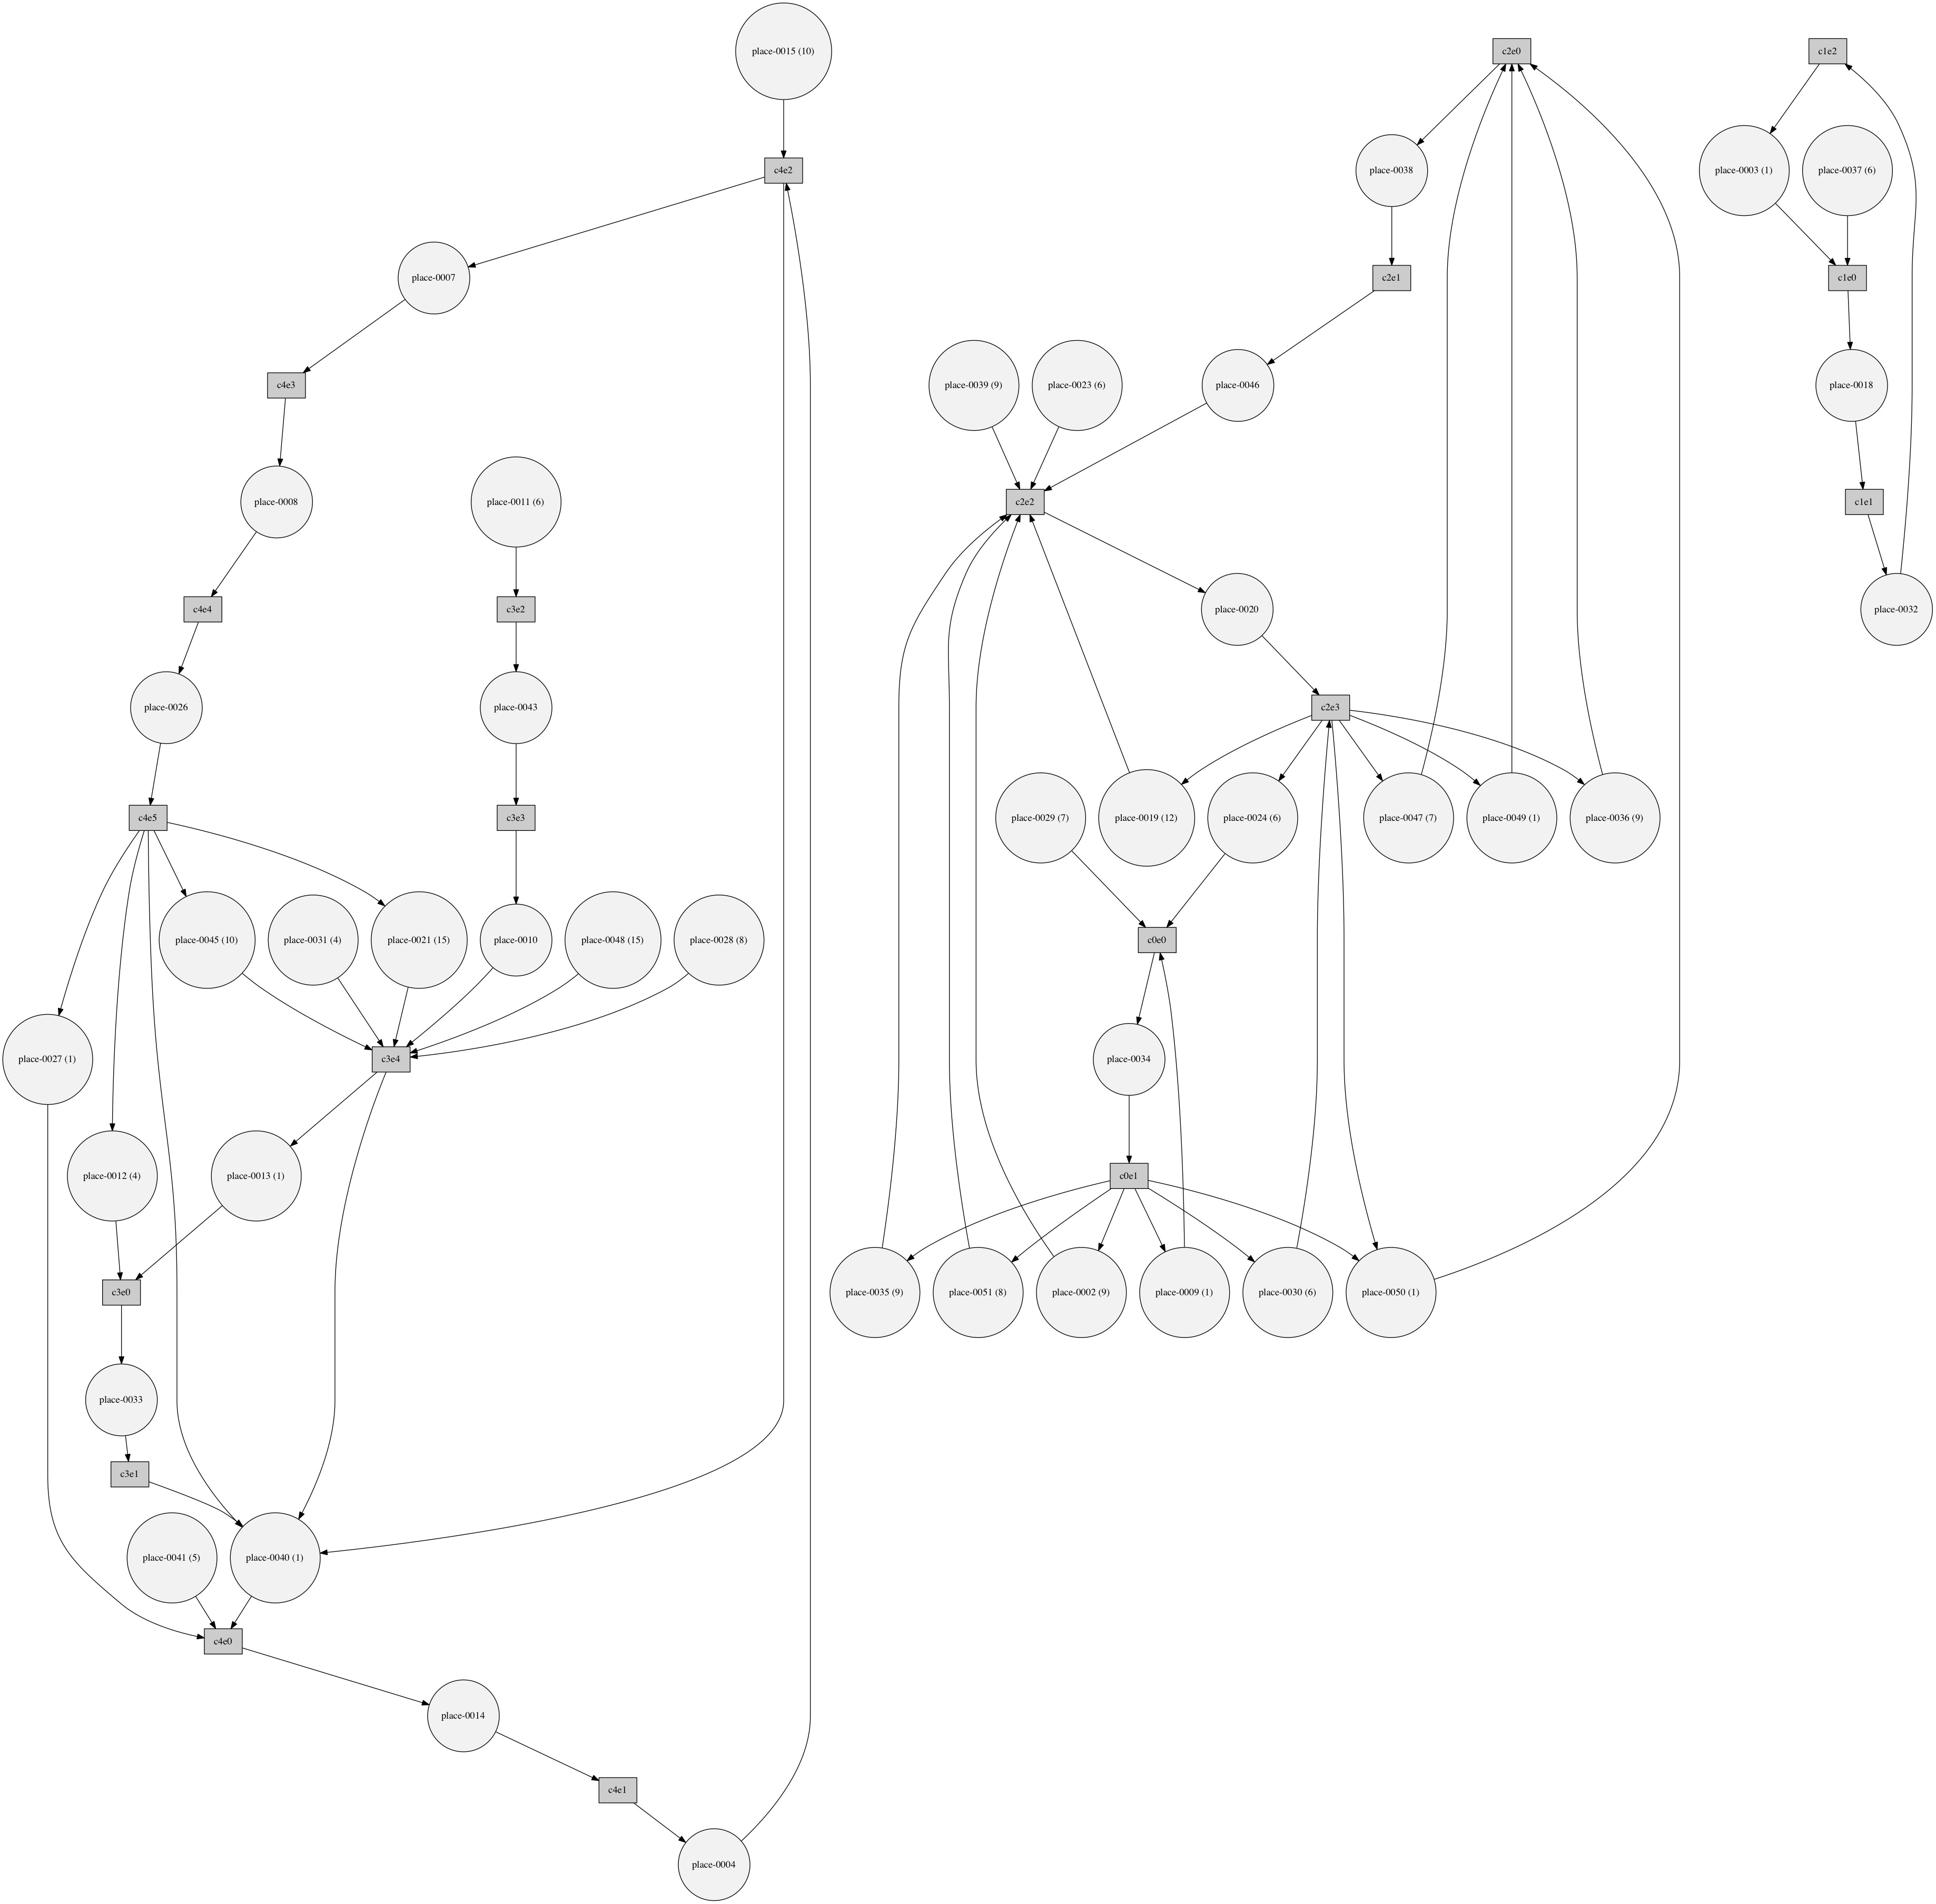
\includegraphics{img/cycles_pnsimp}}}
    \label{fig:allsimp}
    \caption{Ejemplo de la aplicación de la técnica presentada.}
\end{figure}

Los resultados experimentales realizados mediante \pachtool sobre diferentes logs, tanto 
artificiales como reales, avalan la efectividad de la técnica presentada.
Estos resultados se repiten, tanto al utilizar \pachtool como un algoritmo de descubrimiento 
como al ser utilizada como una técnica de post procesamiento sobre modelos existentes.

Se concluye por tanto, que la técnica presentada conjuntamente con la herramienta desarrollada, pueden ser de
gran ayuda en la tarea de derivar modelos de procesos que no solo sean simples, adecuados y precisos, 
sin no que también consistan en una correcta generalización del comportamiento real detrás de un log de eventos.

\section*{Trabajos futuros}

El trabajo realizado está abierto a nuevos aportes, algunos de los que podrían realizarse como 
trabajo futuro se detallan a continuación.

En primer lugar, durante la experimentación se ha inducido información negativa artificial con el fin de obtener 
un log de trazas negativas que permitiese aplicar el proceso supervisado de simplificación. Sería 
interesante contar con la posibilidad de incorporar conocimiento del dominio como información
negativa para simplificar y generalizar modelos utilizando la técnica presentado y estudiar el 
impacto en el modelo final.

En segundo lugar, para esta tesina se ha supuesto que la información negativa se puede separar de la
información positiva proveniente del log de una manera lineal, i.e. mediante un conjunto de semiespacios
que representan un poliedro convexo. Sin embargo, la información negativa puede consistir de puntos negativos en el
interior del poliedro construido. En este caso, la tarea de aprendizaje debe estar orientada no a un único
poliedro sino a un conjunto de poliedros convexos que cubren solamente los puntos positivos, para lo cual
se deberán investigar métodos que unan las soluciones de cada uno de los poliedros.

En tercer lugar, se podrían combinar las técnicas de este trabajo con otras técnicas de simplificación
desarrolladas que enriquecen el modelo con \dquote{valores} -\textit{scores}- de simulación basado en un log~\cite{PedroCC15}.

En cuarto lugar, desde el punto de vista experimental, sería interesante evaluar de manera exhaustiva el impacto de
aplicar las técnicas de simplificación y generalización presentadas sobre diferentes modelos generados mediante otros
algoritmos de descubrimiento.

Por último, como se vio en la~\autoref{sec:4.smthull}, \pachtool permite obtener el poliedro convexo como el resultado de una
codificación de una instancia de SMT obteniendo modelos más eficaces. Sin embargo, este procedimiento posee una limitación
relacionada al tamaño del problema a resolver. Sería interesante intentar sortear esta limitación para obtener una herramienta que
permita generar mejores modelos.

%%%%%%Third, we may combine the techniques of this paper with other simplification techniques developed by some of the
%%%authors that enrich the model with log-based simulation scores. 
